\section{The Project}

\subsection{Introduction}

The \emph{Sidecar container} or \emph{adapter container} or \emph{ambassador container} concept provide a separation and focus on services that reduces spaghetti dependencies and untestable components. Building an application from modular containers means thinking about symbiotic groups of containers that cooperate to provide a service, not one container per service. In Kubernetes, the embodiment of this modular container service is a Pod.\\

A Pod is a group of containers that share resources like file systems, kernel namespaces and an IP address. The Pod is the atomic unit of scheduling in a Kubernetes cluster.

\subsection{schema}

\begin{figure}[ht]
  \caption{sidecar diagram}
  \centering
  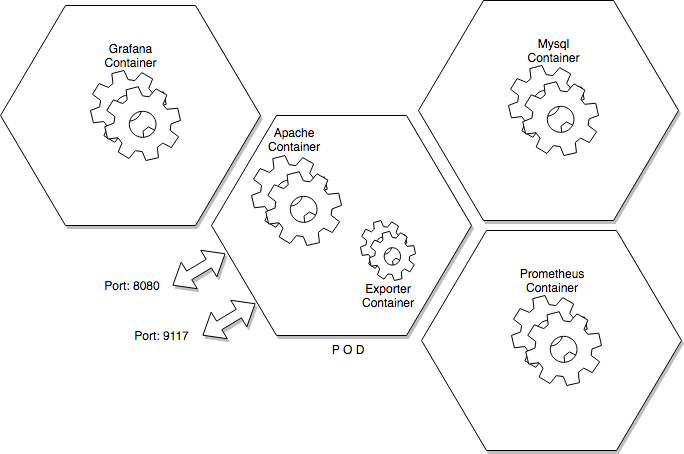
\includegraphics[scale=0.6]{SidecarDiagram.png}
  \label{fig:SidecarDiagram}
\end{figure}

Sidecar containers extends and enhance the \emph{main} container, they take existing container and make them better. As an exemple, consider a container that runs the Apache web server. Add a different container that provide statistics of the system with a exporter and you have built exporter to deploy. But you've done it in a modular manner where the exporter can be built by a different team.

\subsection{Status On Apache}

\emph{status.conf}
\begin{apachecode}
  <Location /server-status>
  SetHandler server-status
  Order deny,allow
  Allow from all
  </Location> ExtendedStatus On>
\end{apachecode}

and  \emph{Dockerfile}

\begin{dockercode}
  FROM ubuntu:latest
  USER root
  ...
  RUN a2enmod status
  COPY status.conf /etc/apache2/mods-enabled/
  EXPOSE 8080
  USER 1001
  CMD ["/usr/sbin/apache2ctl", "-DFOREGROUND"]
\end{dockercode}

\subsection{Secret Access}

We firstly define our \emph{secret file}. If the access is based on a login/password.

\begin{yamlcode}
  apiVersion: v1
  kind: Secret
  metadata:
  name: github-secret
  namespace: sidecar
  type: kubernetes.io/basic-auth
  data:
  username: c3Bpa2U=
  password: dmFsZW50aW5l
\end{yamlcode}

\emph{username} and \emph{password} are defined with the command

\begin{bashcode}
  $ echo -n 'spike' | base64
  c3Bpa2U=
  $ echo -n 'valentine' | base64
  dmFsZW50aW5l
\end{bashcode}

and we run

\begin{bashcode}
  $ oc create -f gitlab-secret.yaml
\end{bashcode}

or if we use a \emph{ssh key},we generate the \emph{key}, create the secret, and link the secret to the right project
\begin{bashcode}
  $ ssh-keygen -C "openshift-source-builder/repo@github" \
  -f repo-at-github -N ''
  $ oc secrets new-sshauth repo-at-github \
  --ssh-privatekey=repo-at-github
$ oc secrets link builder repo-at-github
\end{bashcode}

When we create a new application based on this repository, it desn't work. We have to set the new \emph{build}

\begin{bashcode}
$ oc set build-secret --source bc/mysite repo-at-github
\end{bashcode}

In case of our \emph{GITLAB}, we have to use the login and password based on the \emph{Deploy Tokens}.

\subsection{New Project}

Firstly, we create a new project

\begin{bashcode}
  $ oc new-project sidecar \
  --display-name='Side Car Project' \
  --description='Side Car Project'
\end{bashcode}

\subsection{New Build}

To obtain our image, we firstly
\begin{bashcode}
  $ oc new-build http://192.168.0.8:8880/spike/faye.git \
  --name faye
\end{bashcode}

But to resolve the issue based on the credential, we'll attribute the \emph{login/password} defined before and retstart the build process.

\begin{bashcode}
  $ oc set build-secret --source bc/faye github-secret
  $ oc start-build faye
\end{bashcode}

or directly
\begin{bashcode}
  $  oc new-build http://192.168.0.8:8880/spike/faye.git \
  --source-secret github-secret
  --name faye
\end{bashcode}

\subsection{New Application}

It's time to create our application

\begin{bashcode}
  $ oc new-app faye \
  --name fayeapp
  $ oc status
  $ oc expose service faye
  $ oc get pod
  $ oc get all name --selector app=cdnselect
\end{bashcode}

\section{The Side Car}

\subsection{Export}

We firstly export our \emph{project}.

\begin{bashcode}
  $ oc get --export is,bc,dc,svc -o yaml > export.yaml
\end{bashcode}

\subsection{ImageStream}
We delete \emph{resourceVersion, selfLink and uid}. In status, we keep dockerImageRepository (set to "")

\subsection{BuildConfig}
We delete \emph{resourceVersion, selfLink and uid}. We delete in spec.triggers.imageChange \emph{lastTriggeredImageID}

\subsection{DeploymentConfig}
We replace spec.template.spec.containers.image by \emph{faye} in the first container
We add in spec.template.spec.container

\begin{bashcode}
  - name: apache-exporter
  image: previousnext/apache-exporter
  command: [ "apache_exporter", \
  "-scrape_uri", \
  "http://127.0.0.1:8080/server-status/?auto" ]
  ports:
  - containerPort: 9117
\end{bashcode}

\subsection{Service}
We delete \emph{resourceVersion, selfLink and uid}.

We add in spec.ports

\begin{bashcode}
  - name: 9117-tcp
  port: 9117
  protocol: TCP
  targetPort: 9117
\end{bashcode}

\section{Geek Method}
An other solution concists to create the application without the sidecar, and at the end, we modify the \emph{DeploymentConfig} and \emph{Service}.

\subsection{DeploymentConfig}

The \emph{DeploymentConfig} to add the \emph{exporter-apache} image
\begin{bashcode}
$ oc get dc
$ oc edit dc/faye
\end{bashcode}

\begin{yamlcode}
  spec:
    containers:
        - command:
            - apache_exporter
            - '-scrape_uri'
            - 'http://127.0.0.1:8080/server-status/?auto'
          image: previousnext/apache-exporter
          imagePullPolicy: Always
          name: apache-exporter
          ports:
            - containerPort: 9117
              protocol: TCP
        - image: 172.30.220.103:5000/.......
          imagePullPolicy: Always
          name: faye
          ports:
            - containerPort: 8080
              protocol: TCP
          resources: {}
          terminationMessagePath: /dev/termination-log
          terminationMessagePolicy: File
\end{yamlcode}

The modification of the \emph{DeploymentConfig} will be followed by a  new \emph{build} of the image.

\subsection{Service}

In the common case, we don't have to modify the service, but in this case, we must access to the exporter service through the port \emph{9117}. 
\begin{bashcode}
  $ oc getsvc
  $ oc edit svc/faye
\end{bashcode}

\begin{yamlcode}
spec:
  ports:
    - name: 8080-tcp
      port: 8080
      protocol: TCP
      targetPort: 8080
    - name: 9117-tcp
      port: 9117
      protocol: TCP
      targetPort: 9117
\end{yamlcode}